\section*{Informations générales}
 
\begin{table}[H]
\centering
	\begin{tabularx}{16.8cm}{|X|X|}
	\hline
	 Numéro de l'opportunité & Type de l'opportunité \\
	\hline
	 002 & Livrable terminé en avance  \\
	\hline
	\end{tabularx}
\end{table}

\begin{table}[H]
\centering
	\begin{tabularx}{16.8cm}{|X|X|X|}
	\hline
	Date & Visa du \RQ & Visa du \CP \\
	\hline
	  & & \\
	\hline
	\end{tabularx}
\end{table}

\begin{table}[H]
\centering
	\begin{tabularx}{16.8cm}{|X|X|X|X|}
	\hline
	 Pilote & Activité WBS & Compte WBS & Phase d'apparition \\
	\hline
	 ATANLEY Kafui & Suivre les Risques et Opportunités & 1.2.3.2 & Fin de Sprint \\
	\hline
	\end{tabularx}
\end{table}

\section*{Description de l'opportunité}

\subsection*{Résumé}
	Le livrable est disponible à l'avance permettant de passer directement à la phase de recette. Ceci permettrait de prendre  de replacer ce temps dans une autre phase.
	
\subsection*{Analyse des causes}
	
	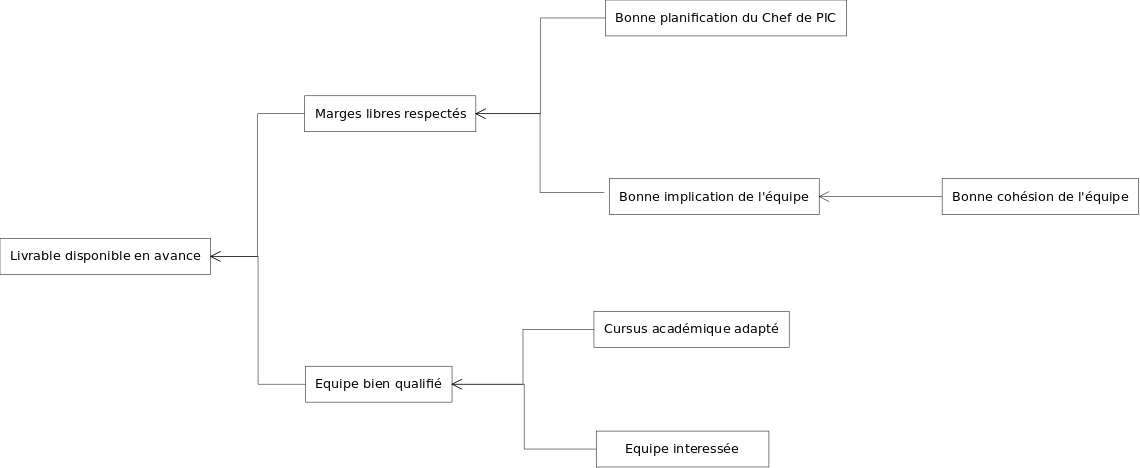
\includegraphics[scale=0.27]{../images/AnalyseOpportunite_nPourquoi_FDO002.png}

\subsection*{Criticité}

\begin{table}[H]
\centering
	\begin{tabularx}{16.8cm}{|>{}X|X|}
	\hline
	Bénéfice & 4\\
	\hline
	Probabilité & 2 \\
	\hline
	Criticité & Important \\
	\hline
	\end{tabularx}
\end{table}

\newpage
\section*{Actions}
\subsection*{Actions proactives}

\centering
	\begin{longtable}{|p{7cm}|p{7cm}|}
	\hline
	Numéro de cause & Actions proactives \\
	
	\hline
	  1 &  \begin{itemize}
	  	\item Entretien individualisé
	  	\item bonne communication
	  	\end{itemize} \\
	  	
	  \hline
	  2 & \begin{itemize} 
	  \item Team-Building
	  \item Entretien individualisé
	  \end{itemize} \\
	  \hline
	  3 & \begin{itemize} 
	  \item Remonter les problématiques fréquentes rencontrées en PIC à la direction. 
	  \end{itemize} \\
	  \hline
	   4 & \begin{itemize}
	   \item Bonne communication autour du projet. 
	   \end{itemize} \\
	\hline
	
\end{longtable}